%\VignetteIndexEntry{Bpest data}
%\VignetteDepends{Bpest}
%\VignettePackage{Bpest}

\documentclass[12pt]{article}

\usepackage{Sweave}

\textwidth=6.2in
\textheight=8.5in
\oddsidemargin=0.2in
\evensidemargin=0.2in
\headheight=0in
\headsep=0in

\begin{document}
\Sconcordance{concordance:vignette.tex:vignette.Rnw:%
1 49 1 1 2 1 0 2 1 26 0 1 1 20 0 1 2 7 1 1 4 3 0 1 1 37 0 1 2 5 1 1 2 5 %
0 1 2 6 1}


\title{Bpest}
\author{Conrad Burden, Sylvain For\^et, Peijie Lin}
\date{\today}
\maketitle

Many of the known mechanisms driving gene regulation fall into the category of epigenomic modifications.
DNA methylation is a common epigenomic modification, in which a cytosine (C) in the genomic DNA sequence can be altered by the addition of a methyl group.
Methylation patterns can be are detected by treating DNA with bisulphite, which converts unmethylated cytosines to uracils while leaving methylated cytosines intact.
This can be carried out at specific loci in a genome by amplifying fragments of interest by PCR.
These PCR products (called amplicons) can be mapped to a reference and methylation patterns inferred. 

However, the bisulphite conversion is not 100\% efficient, and this introduces errors in the observed distribution of methylation patterns.
A second source of errors is the sequencing error.
{\tt Bpest} (for \textbf{B}isulphite \textbf{p}attern \textbf{est}imator)~\cite{Lin04} calculates the estimated distribution over methylation patterns based on an input of methylation pattern count data, an incomplete conversion rate and site-dependent read error rates.

The main component of the package is the function {\tt estimatePatterns()}, which generates a table of estimates $\hat\theta_i$ of the distribution over methylation patterns, and a list of patterns identified as spurious.
Input to the function is a data frame listing the methylation patterns in the first column followed by a number of columns of count data (one column per sample). 
Estimation will be performed on all columns by default unless specified by the variable {\tt column}. The non-conversion and sequencing error rates are specified by the parameters {\tt epsilon} and {\tt eta} respectively. 
The parameter {\tt eta} can be specified globally or as a site-dependent 
array with length equal to the number of CpG sites in the amplicon. 
The boolean variable {\tt fast} enables either a fast implementation (default) which ignores those patterns for which the observed read count is zero or a slow implementation.
The parameter {\tt steps} is passed to the function {\tt constrOptim()} to control the accuracy of the determination of the maximum log-likelihood.

A second function in the package is {\tt plotMethylationPatterns()}. 
Input to this function is a data frame, obtained from the output of {\tt estimatePatterns()}. 
The output of {\tt plotMethylationPatterns()} is a plot that compares the observed read distribution with the estimated distribution.
The parameters {\tt yLimit1} and  {\tt yLimit2} control the range of the y-axis on the plots produced.

In the following example, the input is the table of counts {\tt patternsExample}.
We analyse the second column.
The parameter {\tt epsilon} is 0.01, while the parameter {\tt eta} is not specified and by default is 0. 

\begin{Schunk}
\begin{Sinput}
> library(Bpest)
> data(patternsExample)
> patternsExample
\end{Sinput}
\begin{Soutput}
   mPattern  k1   k2
1    m00000 629 2257
2    m00001  26   90
3    m00010  20   75
4    m00011   2    3
5    m00100  24   82
6    m00101   3    0
7    m00110   1   11
8    m00111   0    0
9    m01000  23   80
10   m01001   0    0
11   m01010   1    1
12   m01011   0    0
13   m01100   1    5
14   m01110   0    0
15   m10000  28   69
16   m10001   1    2
17   m10010   0    2
18   m10011   0    0
19   m10100   0    7
20   m11000   3    1
21   m11001   0    0
\end{Soutput}
\begin{Sinput}
> estimatePatterns(patternsExample, epsilon=0.01, column=2)
\end{Sinput}
\begin{Soutput}
   Pattern Coverage observedDistribution estimatedDistribution Spurious
1    00000     2257         0.8405959032          0.8839245649    FALSE
2    00001       90         0.0335195531          0.0254455613    FALSE
3    00010       75         0.0279329609          0.0202696843    FALSE
4    00011        3         0.0011173184          0.0005775861    FALSE
5    00100       82         0.0305400372          0.0226218133    FALSE
6    00110       11         0.0040968343          0.0035829509    FALSE
7    01000       80         0.0297951583          0.0217709103    FALSE
8    01010        1         0.0003724395          0.0000000000     TRUE
9    01100        5         0.0018621974          0.0013262456    FALSE
10   10000       69         0.0256983240          0.0179381554    FALSE
11   10001        2         0.0007448790          0.0002199047    FALSE
12   10010        2         0.0007448790          0.0002226042    FALSE
13   10100        7         0.0026070764          0.0021000190    FALSE
14   11000        1         0.0003724395          0.0000000000     TRUE
\end{Soutput}
\end{Schunk}

Note that in this example two patterns have been identified as spurious; they are patterns {\tt 01010} and {\tt 11000}.

The following example uses the same input table. 
The {\tt column} variable is not specified, 
so the function {\tt estimatePatterns()} by default applies to both columns of counts.
The sequencing error rate {\tt eta} is specified as a site-dependent array. 

\begin{Schunk}
\begin{Sinput}
> estimates <- estimatePatterns(patternsExample,
+                  epsilon=0.01, 
+                  eta=c(0.008, 0.01, 0.01, 0.01, 0.008))
> estimates
\end{Sinput}
\begin{Soutput}
[[1]]
   Pattern Coverage observedDistribution estimatedDistribution Spurious
1    00000      629          0.825459318          0.9086155891    FALSE
2    00001       26          0.034120735          0.0200619130    FALSE
3    00010       20          0.026246719          0.0100523143    FALSE
4    00011        2          0.002624672          0.0018028445    FALSE
5    00100       24          0.031496063          0.0155874563    FALSE
6    00101        3          0.003937008          0.0030043039    FALSE
7    00110        1          0.001312336          0.0004632978    FALSE
8    01000       23          0.030183727          0.0142452917    FALSE
9    01010        1          0.001312336          0.0004838187    FALSE
10   01100        1          0.001312336          0.0003786940    FALSE
11   10000       28          0.036745407          0.0220014017    FALSE
12   10001        1          0.001312336          0.0002860781    FALSE
13   11000        3          0.003937008          0.0030169970    FALSE

[[2]]
   Pattern Coverage observedDistribution estimatedDistribution Spurious
1    00000     2257         0.8405959032          0.9257131882    FALSE
2    00001       90         0.0335195531          0.0183938459    FALSE
3    00010       75         0.0279329609          0.0115768498    FALSE
4    00011        3         0.0011173184          0.0002218223    FALSE
5    00100       82         0.0305400372          0.0141056682    FALSE
6    00110       11         0.0040968343          0.0033324517    FALSE
7    01000       80         0.0297951583          0.0127610644    FALSE
8    01010        1         0.0003724395          0.0000000000     TRUE
9    01100        5         0.0018621974          0.0009896189    FALSE
10   10000       69         0.0256983240          0.0110531371    FALSE
11   10001        2         0.0007448790          0.0000000000     TRUE
12   10010        2         0.0007448790          0.0000000000     TRUE
13   10100        7         0.0026070764          0.0018523535    FALSE
14   11000        1         0.0003724395          0.0000000000     TRUE
\end{Soutput}
\end{Schunk}

The ouput is a list of two data frames;
now we plot the second data frame.
Two plots are produced: the lower plot is the expanded version of the upper plot.


\begin{Schunk}
\begin{Sinput}
> plotMethylationPatterns(estimates[[2]])
\end{Sinput}
\end{Schunk}
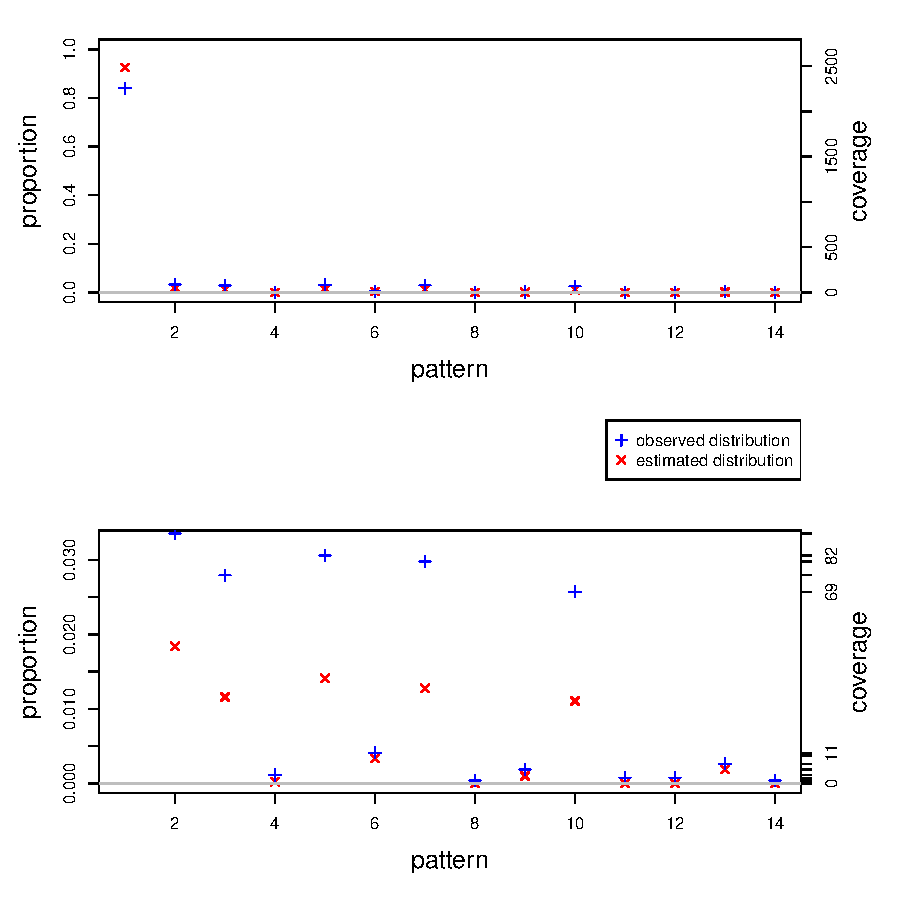
\includegraphics{vignette-003}

\begin{thebibliography}{}
\bibitem{Lin04}
Lin, P., For\^et, S., Wilson, S.R.\ and Burden, C.J., {\it Estimation of amplicon methylation patterns from bisulphite sequencing data} (preprint)
\end{thebibliography}

\end{document}
